\chapter{Background}

In this chapter we compare streaming data flow architectures with
traditional, general purpose architectures and we describe the Maxeler
hardware acceleration solution and the MaxCompiler toolchain and API
which represent the target of the MaxC compilation process. We also
look at the LARA language which will be used as part of the design
flow to specify and apply optimization strategies both to the original
source code and to the resulting dataflow design. We present related
work in the areas of high level synthesis tools, dataflow languages
and aspect-driven compilation for FPGA designs and explain how our
approach differs from existing work in these fields.

\section{Dataflow Computing}

Although general purpose computing devices offer a convenient
programming paradigm, the traditional fetch - decode - execute cycle
is inherently sequential and relies on inefficient access to external
memory. To compensate for this a large area of a modern CPU core is
dedicated to caches, branch prediction units and out-of-order
scheduling and retirement units. This reduces the area of the chip
available for performing useful computation. Furthermore, although
multicore programing is an answer for the processor power wall (which
prevents increases in operating frequency beyond a certain point,
limiting the processing speed of a single core device), there are
classes of algorithms whose performance does not scale linearly with
the number of cores. This is especially true when operating on large
volumes of data with poor spatial locality that do not fit into a
CPU's on-chip cache such as algorithms involving sparse matrix
computations or convolution
\cite{Lindjtorn:Clapp:Pell:Mencer:Flynn:2010}. Although this model
offers good flexibility when dealing with arbitrary access patterns,
it is not efficient for large volumes of highly regular data.

The dataflow computing paradigm operates differently form the general
purpose computing paradigm (as shown in Figure \ref{fig:cpudfe}),
being designed to be efficient at processing large volumes of data. It
works by creating a streaming dataflow graph of computational nodes,
which operates as a large computational pipeline: input data is
streamed in sequentially through each pipeline stage and output data
is streamed out. This results in a highly pipelined design that can be
statically scheduled achieving throughput rates of one value per cycle
by completely avoiding pipeline hazards. This means that a design
running at a few hundred megahertz can outperform a CPU implementation
running at a few gigahertz while being more energy efficient
\cite{Pell:Mencer:2011}.


\begin{figure}[h] \centering
  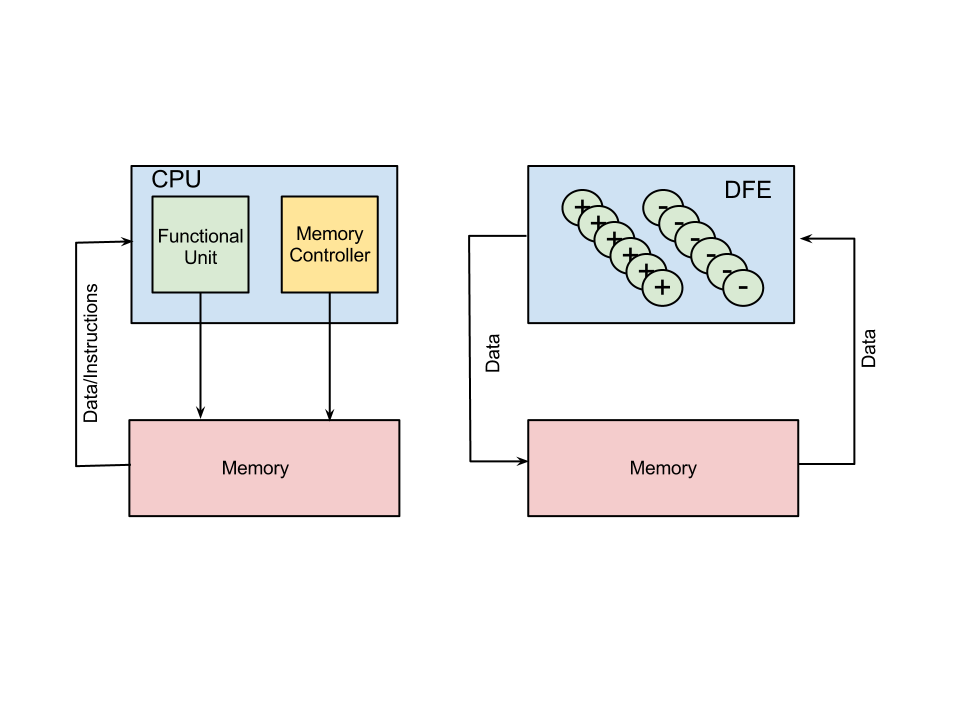
\includegraphics[scale=0.4, trim=0 200 0 150]{figs/cpu-vs-dfe.png}
  \caption{Comparison between general purpose CPU architecture and a
    streaming Data Flow Engine. In the case of the latter instructions are
    not stored in memory but encoded in the dataflow graph. }
  \label{fig:cpudfe}
\end{figure}


\section{FPGA Acceleration}

Dataflow computing is a general computing paradigm that could be
applied to various architectures such as multi-core, GPUs, Cell
processor arrays or ASICs. In this project we chose to focus on FPGAs
for the following reasons:
\begin{itemize}
\item FPGAs provide greater \textbf{flexibility} and lower time-to-market than
  ASICs;
\item FPGAs present exciting \textbf{low-level optimisation opportunities} such
  as word-length optimisations or exploiting run-time reconfiguration
  potential to improve performance at run-time;
\item FPGAs are considerably \textbf{more power efficient} than multi-core CPUs
  and GPUs;
\item FPGAs offer a \textbf{predictable performance model}, due to static
  scheduling and lack of thread barriers or other traditional
  synchronisation mechanisms;
\end{itemize}

One major limitation of FPGAs compared to CPUs and GPUs is the long
development time. This is caused by:
\begin{itemize}
\item \textbf{large compilation time} -- compilation time of a single FPGA
  design can vary from 20 minutes to several days even on multi-core
  clusters with large amount of memory can range from);
\item \textbf{lack of high-level tools} -- although high-level tools such
  as MaxCompiler (\Cref{sec:maxeler-platform} exist that can automate
  the build process and simplify considerably the design of dataflow
  pipelines, these are not high level enough to permit expressing
  algorithms in an intuitive, well-understood approach; additionally
  they do not abstract the underlying hardware architecture, the
  programmer having to constantly deal with adjusting the latency of
  various design components, perform optimisations that allow the
  design to build at higher frequencies etc.;
\item \textbf{large design space} -- this leads to the need to explore a
  large design space which is a time consuming process, especially
  given long compilation times;
\end{itemize}

\subsection{Architecture}

FPGAs are logic chips that can be reconfigured in seconds to implement
custom applications. Hence they offer a much shorter time to market
than traditional ASIC\footnote{Application Specific Integrated
  Circuit} based solutions, while still being able to implement custom
logic circuits, making them significantly faster than general purpose
hardware. However, the size of the FPGA chip constrains the design
that can be uploaded onto the chip. FPGAs have a limited number of
each of the following resource types:

\begin{itemize}
\item \textbf{look-up tables} (LUTs) - implement the logical functions performed by the circuit;
\item \textbf{flip-flops} (FFs) - small storage elements;
\item \textbf{digital signal processors} (DSP) - small special purpose arithmetic units;
\item \textbf{block RAM} (BRAM) - larger, on-chip storage elements.
\end{itemize}

\begin{figure}[ht!]
\centering
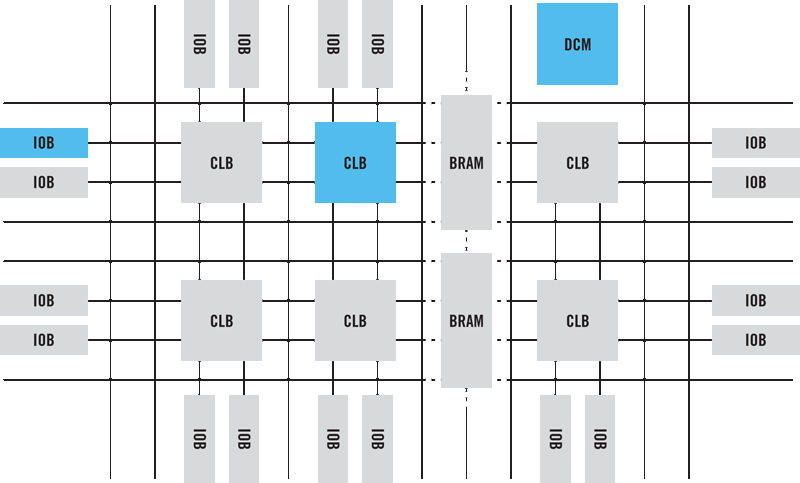
\includegraphics[scale=0.4]{figs/fpga-block-structure.png}
\caption{Structure of an FPGA block: Configurable Logic Blocks (CLB),
  Interconnect, Input/Output Blocks (IOB) and Embedded Memory (BRAM). Source:
  \url{http://www.origin.xilinx.com/fpga/}.}
\label{fig:fpga-block-structure}
\end{figure}

\subsection{Run-time Reconfiguration}
\label{sec:run-time-reconfiguration}
Run-time reconfiguration refers to the capability of uploading a new
design onto the FPGA at run-time. This capability can be used to
maximise usage of the FPGA accelerator for two purposes:
\begin{enumerate}
\item \textbf{enabling} -- to enable the execution of functions that
  would normally not fit on the accelerator; this can be achieved for
  example via time-sharing, where a design is partition into smaller
  tasks that run sequentially on the accelerator\cite{trimberger1998scheduling}
\item \textbf{optimisation} -- to improve performance of FPGA designs,
  by removing idle functions; this can be achieved by removing, at
  run-time, idle portions of a design which allows one to replicate
  the useful functions in order to increase overall performance
\end{enumerate}


For the second type of application we consider the example of a an
FPGA sorting architecture presented in \cite{koch2011fpgasort}. A
parallel sorting tree is used for small problem sizes that fit the
FPGA on-chip memory (a few hundred inputs). While this network
achieves a very high throughput, it does not scale with the number of
inputs, and for larger input sizes it exceeds the available FPGA
resources. Hence, a solution is to combine this network with a
FIFO-based merge sorter\cite{marcelino2009unbalanced} which allows the
merging of sorted buckets of numbers. This leads to a two step sorting
algorithm, using run-time reconfiguration, in which during the first
stage a small number of inputs are merged in parallel and in the
second stage, resulting buckets of inputs are merged to obtain the
final sorted sequence.

An example of the first type of application is shown in
\cite{Xinyu:Qiwei:Luk:Qiang:Pell:2012} run-time reconfiguration is
used to maximise performance by removing idle design components. This
works well in multi-step algorithms such as the Reverse Time Migration
application which has 2 major steps: a forward and a backward
propagation of a simulated wave through the earth surface. Thus the
functions that would only be used in the second stage need not be
uploaded on the accelerator from the very beginning. This enables the
an increase in resources used for the first part which can be used to
increase parallelism and thus reduce computation time.

Based on the reconfiguration technique, we distinguish between
\begin{itemize}
\item \textbf{total reconfiguration}, where the entire FPGA is
  reconfigured with a new design; this exhibits a high reconfiguration
  time often in the are of seconds and requires that data be saved
  from on-board DRAM to host memory during the reconfiguration
  process, which adds significant overhead;
\item \textbf{partial reconfiguration}, where a smaller region of the
  FPGA is reconfigured, reducing reconfiguration overhead, eliminating
  the need for buffering data and minimising computation stall
\end{itemize}

The Maxeler Platform used in this projects was not specifically
designed for run-time reconfiguration. As such it relies on a large
FPGA chip for which the reconfiguration overhead is approximately 0.7
- 1 second, depending on the size of the design. In addition, the slow
data transfer rate and large transfer latency over PCI-Express from
the accelerator card to the memory of the host system introduces
complicates the process of improving performance via run-time
reconfiguration.

The Maxeler Platform does not currently support partial run-time
reconfiguration, so the possibility of using partial run-time
reconfiguration to improve design performance is left as future
work. However, given that partial reconfiguration overhead is smaller
than that of total reconfiguration, our approach will operated
similarly or even better in the case where partial reconfiguration
capabilities are available.

\subsection{Maxeler Platform}
\label{sec:maxeler-platform}
Maxeler Technologies provides a software and hardware acceleration
solution based on the dataflow computing model. The dataflow design is
created using MaxCompiler \cite{Maxeler} and implemented on a specialized
hardware platform, built around high-end Field Programmable Gate Array
(FPGA) chips.


The specific data flow engine used for this project is a MAX3424A card
based on a Virtex 6 FPGA chip \cite{Virtex6}. The MAX3 provides 24GB of
on-board DRAM and about 4MB of fast on-chip BRAM are available on the
FPGA chip.

The system is connected to the dataflow engine via PCIe as shown in
Figure \ref{fig:max3}.

\begin{figure}[h]
  \centering
  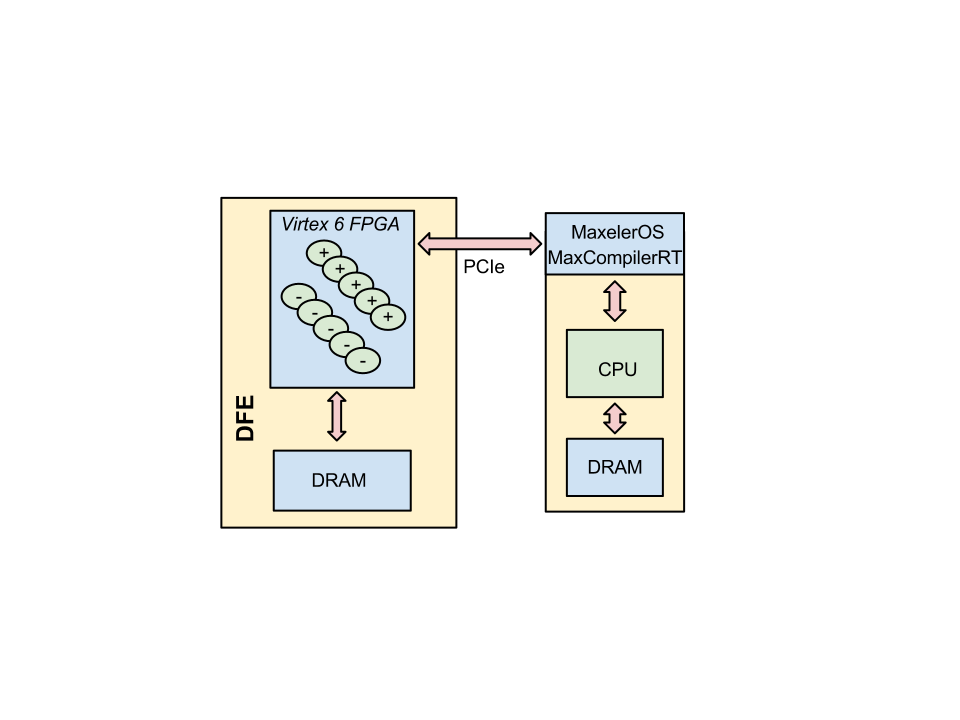
\includegraphics[scale=0.4, trim=0 200 0 200]{figs/max3.png} \caption{
    The Maxeler acceleration solution: the DFE is connected to
    the host machine via PCIe. The board comprises 48GB of DRAM and a
    Virtex 6 FPGA chip. }
  \label{fig:max3}
\end{figure}


Since the target of our compilation process is a MaxJ/MaxCompiler
design, we provide a brief summary of the most important features in
the rest of this section.

We demonstrate the use of MaxCompiler in accelerating a simple moving
average computation, starting from an original design in C shown in
Listing \ref{MovingAvg-C}. This performs a three point moving average
computation on an input array x, using 2 point averages at boundaries.

\begin{lstlisting}[
  language=C++,
  caption={Original three point moving average computation in C.},
  label={MovingAvg-C}]
  for (int i = 0; i < n; i++ ) {
    sum = x[i], divisor = 1;
    if ( i > 0 )
    sum += x[i - 1], divisor++;
    if (i < n - 1)
    sum += x[i + 1], divisor++;
    y[i] = sum / divisor;
  }
\end{lstlisting}

\subsubsection{MaxJ}

MaxJ is a high-level language for specifying dataflow
architectures. It is largely based on Java and adopts a
meta-programming approach for specifying dataflow graphs.  Listing
\ref{lst:moving-avg-kernel} shows the dataflow kernel for computing a
three point moving average over an input stream, which highlights some
of the important features of the MaxJ language:

\begin{itemize}

\item kernel inputs and outputs provide an I/O interface that allow
  the kernel to communicate with the rest of the design (Lines
  \ref{lst:mak-in} and \ref{lst:mak-out});

\item stream offset expressions allow accessing past and future
  elements of a stream (Lines \ref{lst:mak-off} and
  \ref{lst:mak-off2}). The offset window is stored into on chip BRAM
  so is limited to a few tens of thousands elements;

\item frequently used components such as counters are provided by the
  API. They are useful in keeping track of iteration count when
  mapping loops to streaming designs (Line \ref{lst:mak-counter});

\item operator overloading is used to perform arithmetic on input streams;

\item multiplexers (in this instance represented by the overloaded
  conditional operator) are used to select between streams (Lines 11
  and 12).

\end{itemize}

\begin{lstlisting}[
  language=Java, style=MaxJ, label={lst:moving-avg-kernel},
  caption={Kernel design for the three point moving average computation showing features such as stream offsets, arithmetic and control which will have to be supported by our MaxC language}
  ]
  public class MovingAverageKernel extends Kernel{
    public MovingAverageKernel(...) {
      super(...);
      HWVar x = io.input("x", hwFloat(8, 24)); (*@\label{lst:mak-in}@*)
      HWVar cnt = control.count.simpleCounter(32, N); (*@\label{lst:mak-counter}@*)

      HWVar prev = cnt > 0       ? stream.offset(x, -1) : 0; (*@\label{lst:mak-off}@*)
      HWVar next = cnt < (N - 1) ? stream.offset(x, +1) : 0; (*@\label{lst:mak-off2}@*)
      HWVar divisor = cnt > 0 & cnt < (N - 1) ? 3.0 : 2.0;

      HWVar y = (prev + x + next) / divisor;
      io.output("y" , y, hwFloat(8, 24) ); (*@\label{lst:mak-out}@*)
    }
  }
\end{lstlisting}

\subsubsection{MaxCompiler}

\label{sec:back-maxcompiler}

MaxCompiler~\cite{5719584} is a high level compiler targeting the
acceleration platform developed by Maxeler Technologies. It provides a
Java based API for specifying hardware designs that are compiled and
uploaded onto the DFE and a C runtime interface (MaxCompilerRT and
MaxelerOS shown in Figure \ref{fig:max3}) for the part of the
application running on the CPU of the host system.

In addition to the dataflow kernels, a MaxCompiler design also
contains a manager design which is sude manage kernel I/O, connecting
multiple kernels together (in multi kernel designs) and kernels to
DRAM and the CPU interface (via PCIe).

A number of dataflow kernels are connected via a manager to create a
dataflow design which is then compiled to the a Xilinx bitstream that
can be uploaded to the FPGA. Additionally a number of run-time
functions are generated that can be called by the MaxCompiler run-time
to load the design and initiate the streaming of data to and from the
dataflow design.

An example manager design is shown Listing
\ref{lst:moving-avg-manager} and is used to instantiate a single
moving average kernel and connect its inputs and outputs to the host
interface.

\begin{lstlisting}[
  language=Java,
  label={lst:moving-avg-manager},
  caption={Manager design for the
    three point moving average computation}
  ]
  public class MAManager extends CustomManager {
    public MovingAverageManager(...) {
      super(...);
      KernelBlock k = addKernel(new MovingAverageKernel(...));
      k.getInput("x") <== addStreamFromHost("x");
      addStreamToHost("y") <== k.getOutput("y");
    }
  }
\end{lstlisting}

\subsubsection{Run-time}
Finally we must write a host application which is required to queue
the input streams and run the accelerator. This is achieved by calls
to the MaxCompilerRT (runtime) API that interfaces with MaxelerOS.

\begin{lstlisting}[
  label={MovingAverage-Host},
  caption={Host example for queueing
    the input and output streams and running the three point moving
    average design.}
  ]
  max_run(
  device,
  max_input("x", x, x_size),
  max_output("y", y, y_size),
  max_runfor("MAKernel", n),
  max_end());
\end{lstlisting}

\subsubsection{Analysis}
Although the MaxCompiler toolchain greatly simplifies the process of
accelerating applications and particularly the designing of dataflow
kernels, the acceleration process is still very involved and requires
a large amount of experience with FPGA technology and domain specific
knowledge. Most importantly the whole process is manually driven
including the exploration of optimizations. This step is a critical
and time consuming part of the design process which is vital in
achieving maximum performance (in terms of operating frequency, number
of parallel pipelines etc.) subject to physical limitations such as
chip size or timing constraints.

By specifying the design in \FAST{} and optimization strategies in LARA
we aim to create the basis of a design space exploration flow that can
automate this process.

\section{Stencil Computation}
\label{sec:stencil-comp}
Stencil computation is a class of computational problems consisting of
iterative kernels that update array elements based on the values of
their neighbours. The pattern of operation is called a stencil.

Stencil computation has important applications in solving Partial
Differential Equations and computer simulations (such as heat
diffusion).

They can operate on multiple dimensions. But increasing the dimension
heavily impacts memory reference locality, so higher order stencils
are hard to compute on CPU and have been the focus of many
optimisations.

We present some background on a number of applications that can be
reduced to 1, 2 or 3D stencil computation that are used as part of our
benchmark suite (\Cref{sec:benchmark}). We illustrate the importance
of the applications and traditional approaches to accelerating them.

\subsection{Numerical Differentiation}
\label{sec:num-diff-back}
For an example of a 1D stencil we consider the problem of numerical
differentiation \cite{lyness1967numerical}, which provides a method for
estimating the derivative of a function based on its values at
discrete points. By replacing the derivative with finite difference
expressions the following 5 point linear stencil can be derived to
approximate the value of $f'(x)$:

\begin{equation}
  f'(x) = \frac{-f(x + 2h) + 8f(x+h) - 8f(x-h) + f(x - 2h)}{12h}
\end{equation}

Such an approximation is useful for computing the derivative of a
function based on a discrete set of observed values (e.g. to compute
speed/acceleration of an object based on a discrete sample of
displacements/speeds). It provides better accuracy at the cost of
double computational cost when compared to Newton's difference
quotient $f'(x) = \frac{f(x + h) - f(x)}{h}$ or the slope of secant
method $f'(x)=\frac{f(x+h) - f(x - h)}{2h}$.

Hence the following stencil algorithm could be used to compute the
numerical approximation of the derivative of $f$ for a large number of
points in the function's domain:

\begin{algorithm}
  \caption{Stencil approximation of first order derivative}
  \begin{algorithmic}
    \Function{NumericalDifferentiation}{$f, Order$}
    \State $h \gets \epsilon$
    \For{$x \in {Order, nPoints - Order}$}
    \State $f'(x) \gets  \frac{-f(x + 2h) + 8f(x+h) - 8f(x-h) + f(x - 2h)}{12h}$
    \EndFor
    \State \Return $f'$
    \EndFunction
  \end{algorithmic}
\end{algorithm}

\subsection{Black Scholes Equation}

Stencil computation can also be used for solving Partial Differential
Equations using finite difference methods. This has many applications
in scientific computing for finance and physics for example, where
PDEs are used to model the dynamic behaviour of a system. For example,
the solution to the widely-used Black Scholes equation can be
approximated using a 2D stencil computation.

\begin{equation}
  \frac{\partial V}{\partial t} + \frac{1}{2}\sigma^2S^2\frac{\partial^2 V}{\partial S^2} + rS\frac{\partial V}{\partial S} -rV = 0
\end{equation}

where:
\begin{itemize}
\item S - stock price,
\item V(t, S) - price of derivative as a function of stock price and time
\item r - risk-free interest rate
\item $\sigma$ - volatility of the stock's returns
\end{itemize}

A finite difference approximation using the explicit method leads to a
recursive formula \cite{blackscholes} for $v(i, j)$, the approximated
value of $V$ at the $i$th point in the time dimension and the $j$th
point in the stock price dimension:

\begin{equation}
  v(i, j) =
  \alpha * v(i, j - 1) +
  \beta  * v(i, j) +
  \gamma * v(i, j + 1)
\end{equation}

This leads to a 2D stencil algorithm that performs a forward
propagation on the time parameter by iteratively computing the values
of $v(i + 1, j)$ for all $j$, given the values of $v(i, j)$ for all
$j$ as show in Algorithm \ref{alg:bscholes-stencil}.

\begin{algorithm}
  \caption{Stencil kernel for finite difference approx. of Black Scholes PDE}
  \label{alg:bscholes-stencil}
  \begin{algorithmic}
    \Function{BlackScholes}{payoff, timesteps}
    \For{i $\in$ {0, timesteps}}
    \For{j $\in$ {1, size(payoff) - 1} }
    \State payoff\_next[j] $\gets$ $\alpha *$ payoff[j$ -1$] $+ \beta *$ payoff[j] $ + \gamma * $ payoff[j$ + 1$]
    \EndFor
    \State payoff $\gets$ payoff\_next
    \EndFor
    \State \Return payoff
    \EndFunction
  \end{algorithmic}
\end{algorithm}

Although the shape of the stencil remains one dimensional, by contrast to
the numerical differentiation example, the computation is also
propagated forward in time, adding another (time) dimension. Thus this
can be viewed as a 2D computation.

%\subsection{Edge Detection}

Edge detection algorithms can be used to detect points at which sudden
changes in image brightness occur. These images

\subsection{Reverse Time Migration}
\label{sec:rtm-back}
Stencil computation is also used for advanced simulation and imaging
algorithms. For example the Reverse Time Migration technique is used
to detect geological structures beneath the Earth's
surface~\cite{baysal1983reverse} and is widely used in the Oil and Gas
sector. The algorithm uses a forward propagation step which models the
propagation of injected acoustic waves with the isotropic acoustic
wave equation~\cite{araya2011assessing}:
\begin{align}
  \frac{d^2p(r,t)}{dt^2} + {c(r)}^2\bigtriangledown^2p(r,t) = f(r,t)
\end{align}
where:
\begin{itemize}
\item c(r)    - sound speed model
\item p(r, t) - seismic wave value at point r, time t
\item f(r, t) - input wave value at point r, time t
\end{itemize}

An approximation using finite difference is given in
\cite{xinyu2013selfaware} and leads to the 3D stencil kernel
\cite{Xinyu:Qiwei:Luk:Qiang:Pell:2012} shown in Algorithm
\ref{algo:sten}.
\begin{algorithm}[!ht]\footnotesize
  \caption{Stencil Kernel for Reverse Time Migration.}
  \label{algo:sten}
  \begin{algorithmic}
    \For{$t$ = 0 $\leftarrow$ nt-1}
    \For{$x$ = 0 $\leftarrow$ nx-1}
    \For{$y$ = 0 $\leftarrow$ ny-1}
    \For{$z$ = 0 $\leftarrow$ nz-1}
    \State p(t,x,y,z) = c *(
    \State c0 * p(t,x,y,z) +
    \State c11* (p(t,x-1,y,z) + p(t,x+1,y,z)) + ... + c15*(p(t,x-5,y,z) + p(t,x+5,y,z)) +
    \State c21* (p(t,x,y-1,z) + p(t,x,y+1,z)) + ... + c25*(p(t,x,y-5,z) + p(t,x,y+5,z)) +
    \State c31* (p(t,x,y,z-1) + p(t,x,y,z+1)) + ... + c35*(p(t,x,y,z-5) + p(t,x,y,z+5)) +
    \State d0 *  p(t,x,y,z) + d1 * p(t-1,x,y,z-1) + f(t,x,y,z);
    \EndFor
    \EndFor
    \EndFor
    \EndFor
  \end{algorithmic}
\end{algorithm}


\section{Aspect Oriented Programming}

Aspect-Oriented Programming \cite{Kiczales:2005:AP:1062455.1062640} is
a programming paradigm which is used to capture aspects that cut
through levels of abstractions. A commonly used example is that of
program logging \cite{jacobson2004aspect}, which represents a concern
that is expressed at, for example, every method entry and exit
point. The functions that perform logging are spread throughout the
code and, for example, ensuring consistency when changing the logging
format can be difficult. Encapsulating crosscutting concerns in
aspects can improve cohesion, making the code easier to understand and
change which leads to improved maintainability and increased developer
productivity. The model which governs the application of aspects to
code is named \emph{join-point model} and describes where in the
application (the \emph{pointcut}) should the functionality implemented
in the aspect (the \emph{advice}) be applied.

This idea can also be applied to the compilation of dataflow designs,
by regarding the optimisations and transformations that are applied to
the original design as cross-cutting concerns. These optimisations can
often hide the original purpose of the application, making it harder
to maintain and by encapsulating them in aspects we not only improve
the maintainability of the application but also simplify the process
of optimisation and take important steps towards fully automating the
optimisation and transformation process.

However, most commonly used implementations of Aspect-Oriented
Programming, such as AspectJ \cite{Gradecki:Lesiecki:2003,
  Kiczales:2001} and AspectC++\cite{Spinczyk:Gal:Schroder:2002} share
a limitation which makes them impossible to use for capturing design
optimisations and transformations, without substantial extensions:
aspects cannot be applied to multiple statement blocks, loops or
conditionals.

Hence, for the purpose of this project we use LARA, an Aspect-Oriented
Programming language that was introduced in the scope of the
REFLECT\cite{Cardoso:Bertels:Kuzmanov:Nane:Sima:2011} project, also to
support the process of optimising FPGA designs.

\subsection{LARA}

Lara is an Aspect-Oriented Programming language for specifying
compiler strategies for FPGA-based systems
\cite{Cardoso:Teixeira:Alves:Nobre:Diniz:Cutinho:Luk:2012}. LARA
facilitates decoupling of optimisations from apllication code and
enables the capturing of strategies for:

\begin{itemize}
\item \emph{instrumentation}, \emph{monitoring} and
  \emph{hardware/software partitioning}, used in the initial stages of
  our design flow to identify optimisation candidates for mapping onto
  the dataflow engine

\item code \emph{specialisation} and \emph{optimisation}, used both
  for the original host application and dataflow designs which are the
  input of our design flow
\end{itemize}

Furthermore LARA descriptions can be parametrised to simplify
integration with our proposed design space exploration step described
in Chapter \ref{sec:design-flow}.

Listing \ref{lara} shows an example description used for fully
unrolling all innermost loops with an iteration count smaller than or
equal to 16. The `select` statement on line 2 captures the join points
on which the aspect acts, the `apply` statement specifies actions to
be applied to the results of a query while `condition` is used to
filter relevant queries.

\begin{lstlisting}[
  style=lara,
  label={lara},
  caption={Example LARA description
    for fully unrolling innermost loops with an iteration count smaller
    than or equal to 16.}
  ]
  aspectdef loopunroll
  select function.loop{type="for"} end
  apply optimize("loopunroll", "fully"); end
  condition $loop.is_innermost && $loop.num_iter<=16; end
  end
\end{lstlisting}

\cite{Cardoso:Carvalho:Teixeira:Diniz:Goncalves:Petrov:2012} also
introduces a design flow based on LARA for mapping applications into
heterogeneous multi-core platforms. This involves specifying
optimisations and mapping strategies in the LARA programming language,
separate from the application source code.

The strategies are compiled and applied to the original source code in
a sequential order to obtain the final design which is synthesised
using Catapult-C \cite{CatapultC}. Examples of strategies which are
expressed using LARA include loop unrolling, coalescing, loop fission
and mapping compute intensive functions to hardware (hardware/software
partitioning).

Advantages of the aspect based approach compared with the popular
pragma based approach used in frameworks like
OpenMP \cite{Ferrer:Judit:Bellens:Duran:Gonzalez:Marorell:Badia:Ayquade:Labarta:2011}
include the possibility of defining dynamic join points through which
strategies can be applied to the intermediate results of the weaving
(source translation) process. Additionally, optimisation strategies are
grouped into cohesive aspects, rather than being spread through the
code which makes them easier to understand, maintain and modify, for
example to target a different platform.


\section{Related Work}

\subsection{High Level Synthesis}

Substantial work has been carried out in synthesising high level
languages to hardware designs and many tools exist for this purpose
\cite{CtoVerilog, Vivado, ImpulseC}. However these approaches
do not target a streaming dataflow architecture but either soft
processor designs - processor cores implemented on the FPGA chip with
configurable custom computing units (e.g. floating point units). These
usually offer limited speedups when compared to high-end hardcore
CPUs but can turn out to be more energy efficient.

\cite{Czerniawski} proposes a method for synthesising hardware
pipelines from OpenCL programs which exploits some important concepts
related to parallelism exposed by the OpenCL specification
\cite{OpenCL} such as threads and domain decomposition into threads
sharing local memory. Although we are dealing with simple C kernels
for this project, some of the proposed compilation strategies can be
applied for loops.

\subsection{Dataflow Languages}
A number of dataflow languages have been developed targeting FPGAs but
also multi-core platforms.

Lucid~\cite{ashcroft1977lucid} (implemented in \cite{pLucid}),
SISAL~\cite{gurd1987implicit,mcgraw1983sisal}, and
Lustre~\cite{halbwachs1991synchronous}, are examples of functional
dataflow languages. The latter is based on a synchronous programming
model, facilitating safety verification for critical
software~\cite{halbwachs1992programming} rather than performance. The
functional programming style complicates the translation of existing
imperative applications and none have existing implementations for
FPGAs, so a performance comparison is not possible. Control flow
extensions to dataflow languages have also been investigated in
\cite{143862} and \cite{183202}. This shows that in most real life
applications, it is necessary to specify a control path as well as a
data path.

Streams-C~\cite{Gokhale:Stone:Arnold:Kalinowski:2000} and
ImpulseC~\cite{ImpulseC} adopt imperative ANSI C syntax and an
execution model based on Communicating Sequential Processes and
introduce non-standard syntax and constructs for specifying designs
such as special comment blocks which are used to annotate the C
application code. The specialised syntax makes the languages harder to
integrate with existing source-to-source translation or aspect weaving
frameworks.

Hybrid approaches such as MaxCompiler~\cite{5719584} separate the CPU
run-time component from the accelerated one, providing a C run-time
environment and a Java API for building dataflow designs via
meta-programming. The separation complicates the development process,
hindering sharing of design parameters and, consequently, the design
space exploration process. The use of meta-programming simplifies
design parametrisation, but can make resulting programs harder to
understand. In contrast, the proposed approach allows the computation
description, which includes CPU and dataflow components, to be specified
using a single language and to be decoupled from design
parametrisation and other optimisation strategies which are captured
as LARA aspects. This separation of concerns results in more intuitive
and maintainable descriptions.


\subsection{Aspect-driven Compilation of FPGA Designs}

One attempt at capturing optimisation strategies for FPGA designs
using aspect descriptions is LARA
\cite{Cardoso:Carvalho:Cutinho:Luk:Nobre:Diniz:Petrov:2012,
  Cardoso:Carvalho:Teixeira:Diniz:Goncalves:Petrov:2012}, an Aspect
Oriented language for embedded systems. Aspect descriptions are
written in the LARA language and automatically applied to the
original application source to generate optimised versions through
various transformations that enable and optimise hardware/software
partitioning \cite{Lam:Coutinho:Luk:2008}. Aspect descriptions can be
used to specify compilation strategies that result in overall
speedups of 2 to 6.8 times over software versions
\cite{Cardoso:Teixeira:Alves:Nobre:Diniz:Cutinho:Luk:2012}, generally
with high aspect bloat \footnote{ $\text{aspect bloat} =
  \frac{\text{size of transformed code}}{\text{size of original
      code}}$, so a higher aspect bloat is better}
\cite{Cardoso:Carvalho:Cutinho:Luk:Nobre:Diniz:Petrov:2012}.

The use of LARA aspects in guiding the compilation process of C
applications is described in
\cite{Cardoso:Teixeira:Alves:Nobre:Diniz:Cutinho:Luk:2012} and
\cite{cardoso2011new} but the backend compilation targets a von
Neumann architecture (with a GPP and custom accelerator) unlike the
dataflow architecture proposed in this project. The approach described
in \cite{Cardoso:Teixeira:Alves:Nobre:Diniz:Cutinho:Luk:2012} and
\cite{cardoso2011new} relies more on high-level source transformation
whereas our approach is based on a systematic design space exploration
process, which enables the analysis of more low-level
optimisations. Finally,
\cite{Cardoso:Teixeira:Alves:Nobre:Diniz:Cutinho:Luk:2012} and
\cite{cardoso2011new} do not consider development aspects which can be
used to improve developer productivity.


The use of aspect-oriented programming for specifying strategies for
run-time adaptation of FPGA designs discussed in \cite{6322875}
differs from the static process considered in this paper in which the
application is partitioned and scheduled at compile time, to achieve
optimised performance as described in
\cite{Xinyu:Qiwei:Luk:Qiang:Pell:2012}. An advantage of our approach
is that an optimised allocation is generated prior to application
execution. However, we lack the flexibility of adapting the design to
varying input conditions.

\section{Summary}

We have provided a brief introduction into the area of dataflow
computing and explained why dataflow acceleration can improve
performance and energy efficiency over traditional software only
solutions. We have shown the main benefits and drawbacks of FPGA
acceleration and explained why we have chosen to target custom
streaming architectures with our design flow. We have introduced the
Maxeler platform which will be used as the backend of the compilation
process presented in Chapter \ref{sec:design-flow} and presented some
of the more important features of the MaxCompiler approach including
some limitations that we attempt to address with the proposed flow in
order improve developer productivity and possibly reveal new
opportunities for design transformation and optimisations. As an
example of parallel computation where FPGAs can be used to obtain
substantial speedups we have presented stencil computation. Finally,
we briefly introduced related work in the areas of dataflow languages
and aspect-driven compilation for FPGA designs and shown that our
approach differs from existing work by:

\begin{itemize}
\item introducing a novel approach for generating and optimising
  dataflow designs based on an aspect-oriented compilation flow
\item focusing on separating optimisations from functional application
  code with the view of improving both maintainability and performance
\item focusing on a streaming, high-throughput architecture based on
  FPGA Dataflow Engines
\item introducing explicit support for specifying run-time
  reconfiguration strategies to improve performance and energy
  efficiency
\end{itemize}